% Reusable PGFPlots figures for the living technical report.
% Keep these figures data-light and paper-oriented: they summarize the
% report-ready values already recorded in the corresponding sections.

\newcommand{\ExpFourteenAParetoFigure}{%
\begin{figure}[t]
    \centering
    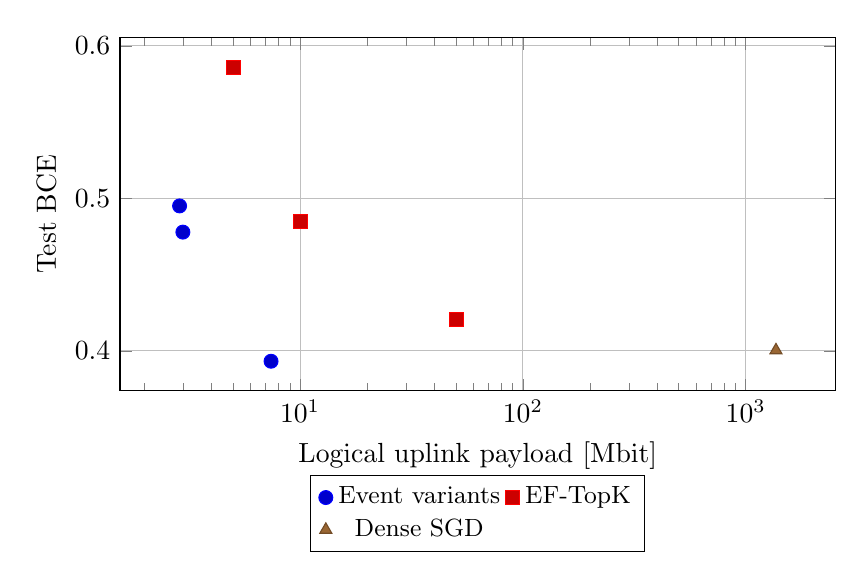
\begin{tikzpicture}
    \begin{axis}[
        width=0.88\linewidth,
        height=0.50\linewidth,
        xmode=log,
        xlabel={Logical uplink payload [Mbit]},
        ylabel={Test BCE},
        grid=major,
        legend style={font=\small,at={(0.5,-0.24)},anchor=north,legend columns=2},
        mark size=2.5pt,
    ]
        \addplot+[only marks,mark=*] coordinates {(2.88,0.49502) (2.98,0.47783) (7.41,0.39317)};
        \addlegendentry{Event variants}
        \addplot+[only marks,mark=square*] coordinates {(5.01,0.58597) (10.01,0.48489) (50.21,0.42059)};
        \addlegendentry{EF-TopK}
        \addplot+[only marks,mark=triangle*] coordinates {(1366.61,0.40033)};
        \addlegendentry{Dense SGD}
    \end{axis}
    \end{tikzpicture}
    \caption{Experiment~14A communication--performance trade-off on the strong non-IID binary Fashion-MNIST task. Lower and further left is better. The selected event operating point reaches the dense predictive regime while remaining far below dense communication.}
    \label{fig:exp14a-pareto}
\end{figure}%
}

\newcommand{\ExpFourteenBSeedFigure}{%
\begin{figure}[t]
    \centering
    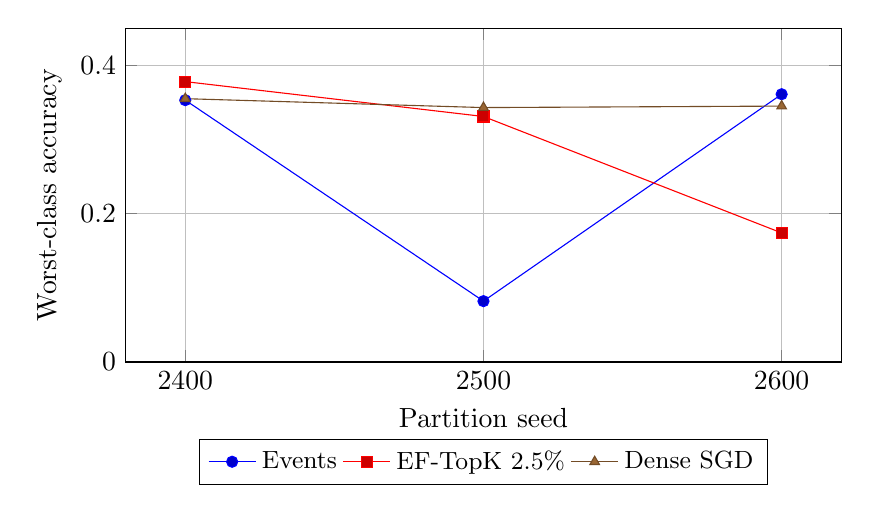
\begin{tikzpicture}
    \begin{axis}[
        width=0.88\linewidth,
        height=0.48\linewidth,
        xlabel={Partition seed},
        ylabel={Worst-class accuracy},
        xtick={1,2,3},
        xticklabels={2400,2500,2600},
        ymin=0,
        ymax=0.45,
        grid=major,
        legend style={font=\small,at={(0.5,-0.23)},anchor=north,legend columns=3},
    ]
        \addplot+[mark=*] coordinates {(1,0.353) (2,0.082) (3,0.361)};
        \addlegendentry{Events}
        \addplot+[mark=square*] coordinates {(1,0.378) (2,0.331) (3,0.174)};
        \addlegendentry{EF-TopK 2.5\%}
        \addplot+[mark=triangle*] coordinates {(1,0.355) (2,0.343) (3,0.345)};
        \addlegendentry{Dense SGD}
    \end{axis}
    \end{tikzpicture}
    \caption{Experiment~14B worst-class accuracy across independent strong-skew partitions at 650 ticks. The seed-2500 event transient is visible immediately, motivating the class-wise and compute-heterogeneity audits in Experiment~14C.}
    \label{fig:exp14b-seed-worst}
\end{figure}%
}

\newcommand{\ExpFourteenCMatchedWorkFigure}{%
\begin{figure}[t]
    \centering
    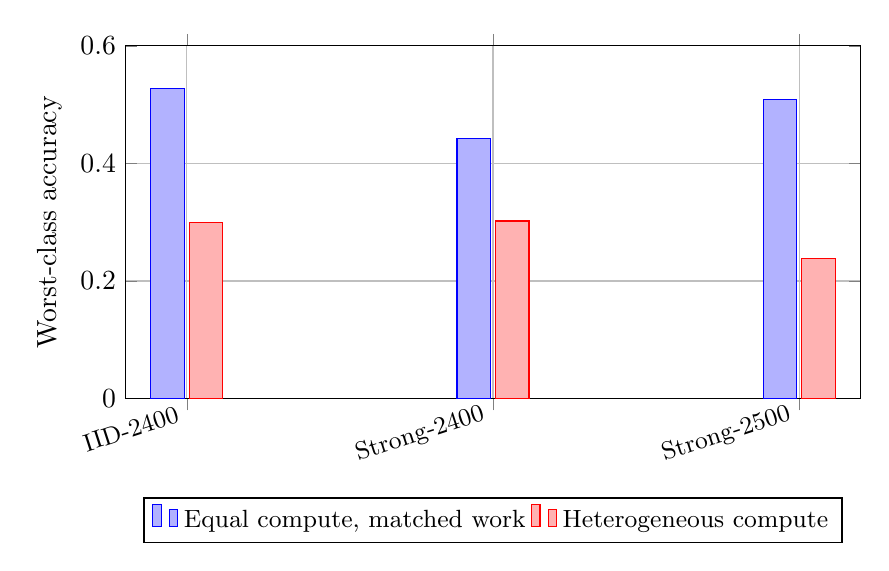
\begin{tikzpicture}
    \begin{axis}[
        width=0.90\linewidth,
        height=0.50\linewidth,
        ybar,
        bar width=12pt,
        ylabel={Worst-class accuracy},
        symbolic x coords={IID-2400,Strong-2400,Strong-2500},
        xtick=data,
        xticklabel style={rotate=18,anchor=east,font=\small},
        ymin=0,
        ymax=0.6,
        grid=major,
        legend style={font=\small,at={(0.5,-0.28)},anchor=north,legend columns=2},
    ]
        \addplot coordinates {(IID-2400,0.528) (Strong-2400,0.443) (Strong-2500,0.508)};
        \addlegendentry{Equal compute, matched work}
        \addplot coordinates {(IID-2400,0.300) (Strong-2400,0.302) (Strong-2500,0.239)};
        \addlegendentry{Heterogeneous compute}
    \end{axis}
    \end{tikzpicture}
    \caption{Experiment~14C matched-work event comparison. Compute heterogeneity materially delays worst-class convergence even when the total number of local completions is controlled.}
    \label{fig:exp14c-matched-work}
\end{figure}%
}

\newcommand{\ExpFifteenAParetoFigure}{%
\begin{figure}[t]
    \centering
    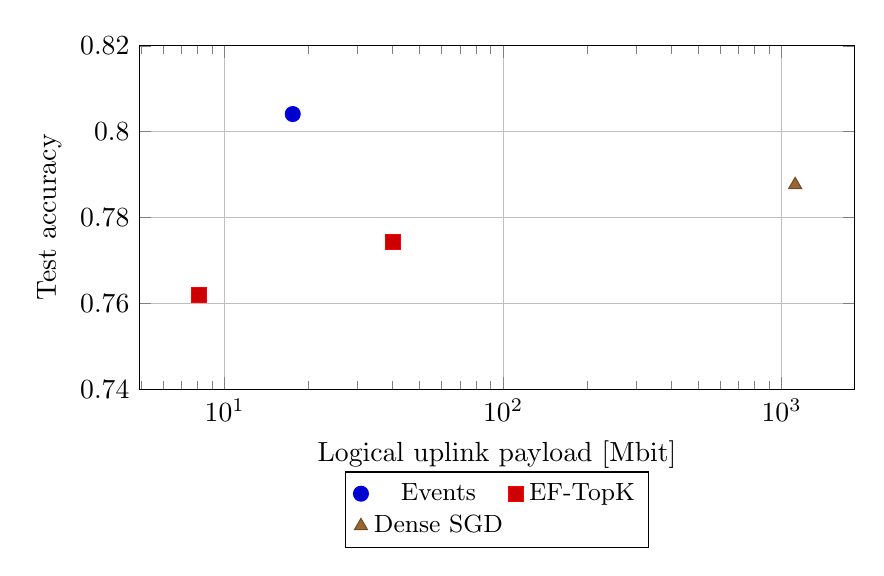
\begin{tikzpicture}
    \begin{axis}[
        width=0.88\linewidth,
        height=0.49\linewidth,
        xmode=log,
        xlabel={Logical uplink payload [Mbit]},
        ylabel={Test accuracy},
        ymin=0.74,
        ymax=0.82,
        grid=major,
        legend style={font=\small,at={(0.5,-0.24)},anchor=north,legend columns=2},
        mark size=2.7pt,
    ]
        \addplot+[only marks,mark=*] coordinates {(17.55,0.8041)};
        \addlegendentry{Events}
        \addplot+[only marks,mark=square*] coordinates {(8.07,0.7619) (40.14,0.7742)};
        \addlegendentry{EF-TopK}
        \addplot+[only marks,mark=triangle*] coordinates {(1118.38,0.7876)};
        \addlegendentry{Dense SGD}
    \end{axis}
    \end{tikzpicture}
    \caption{Experiment~15A compact-CNN operating points at 650 ticks. The raw coordinate-event method remains on a favorable communication--accuracy frontier after convolution and weight sharing are introduced.}
    \label{fig:exp15a-pareto}
\end{figure}%
}

\newcommand{\ExpFifteenAFinalFigure}{%
\begin{figure}[t]
    \centering
    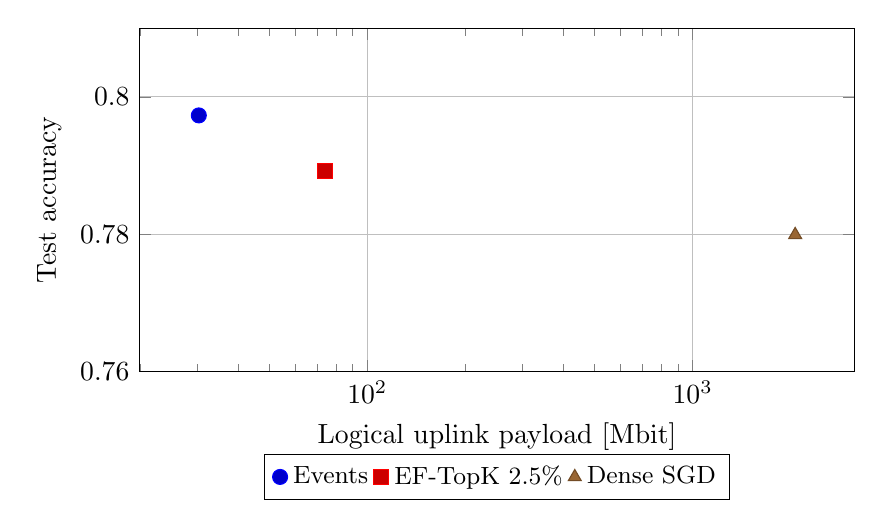
\begin{tikzpicture}
    \begin{axis}[
        width=0.88\linewidth,
        height=0.49\linewidth,
        xmode=log,
        xlabel={Logical uplink payload [Mbit]},
        ylabel={Test accuracy},
        ymin=0.76,
        ymax=0.81,
        grid=major,
        legend style={font=\small,at={(0.5,-0.24)},anchor=north,legend columns=3},
        mark size=2.7pt,
    ]
        \addplot+[only marks,mark=*] coordinates {(30.34,0.7973)};
        \addlegendentry{Events}
        \addplot+[only marks,mark=square*] coordinates {(74.14,0.7892)};
        \addlegendentry{EF-TopK 2.5\%}
        \addplot+[only marks,mark=triangle*] coordinates {(2065.56,0.7799)};
        \addlegendentry{Dense SGD}
    \end{axis}
    \end{tikzpicture}
    \caption{Experiment~15A canonical paired 1200-tick validation after strengthening the event-resolution decay. The selected event schedule recovers competitive long-horizon performance while retaining a large communication reduction.}
    \label{fig:exp15a-final}
\end{figure}%
}

\newcommand{\QTwoCommunicationFigure}{%
\begin{figure}[t]
    \centering
    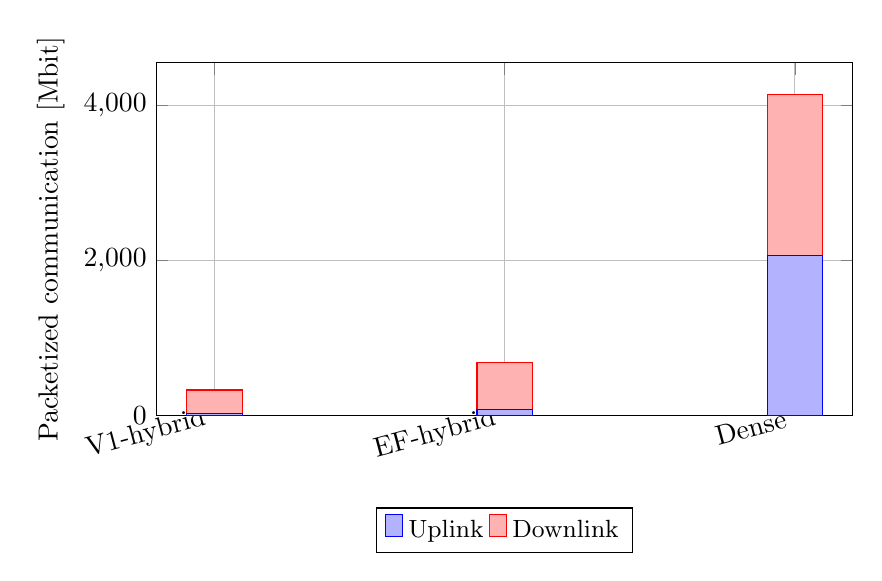
\begin{tikzpicture}
    \begin{axis}[
        width=0.86\linewidth,
        height=0.50\linewidth,
        ybar stacked,
        bar width=20pt,
        ylabel={Packetized communication [Mbit]},
        symbolic x coords={V1-hybrid,EF-hybrid,Dense},
        xtick=data,
        xticklabel style={rotate=15,anchor=east},
        ymin=0,
        grid=major,
        legend style={font=\small,at={(0.5,-0.26)},anchor=north,legend columns=2},
    ]
        \addplot coordinates {(V1-hybrid,30.62) (EF-hybrid,74.42) (Dense,2065.84)};
        \addlegendentry{Uplink}
        \addplot coordinates {(V1-hybrid,300.25) (EF-hybrid,614.28) (Dense,2070.17)};
        \addlegendentry{Downlink}
    \end{axis}
    \end{tikzpicture}
    \caption{Q2 conservative bidirectional communication accounting. Sparse downlink replay with checkpoint fallback preserves the V1 advantage; dense model synchronization would largely mask the uplink savings.}
    \label{fig:q2-bidirectional}
\end{figure}%
}

\newcommand{\QThreeLocalWorkFigure}{%
\begin{figure}[t]
    \centering
    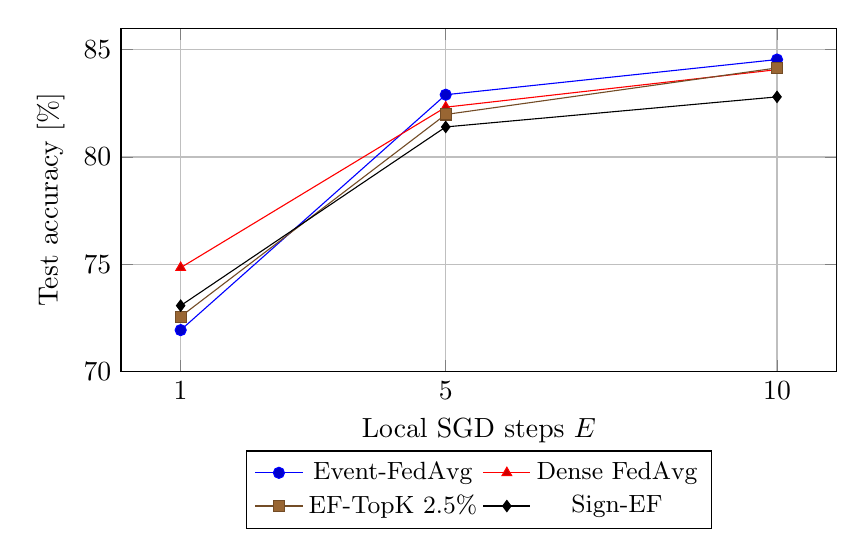
\begin{tikzpicture}
    \begin{axis}[
        width=0.88\linewidth,
        height=0.49\linewidth,
        xlabel={Local SGD steps $E$},
        ylabel={Test accuracy [\%]},
        xtick={1,5,10},
        ymin=70,
        ymax=86,
        grid=major,
        legend style={font=\small,at={(0.5,-0.23)},anchor=north,legend columns=2},
    ]
        \addplot+[mark=*] coordinates {(1,71.93) (5,82.90) (10,84.54)};
        \addlegendentry{Event-FedAvg}
        \addplot+[mark=triangle*] coordinates {(1,74.84) (5,82.32) (10,84.07)};
        \addlegendentry{Dense FedAvg}
        \addplot+[mark=square*] coordinates {(1,72.56) (5,81.98) (10,84.15)};
        \addlegendentry{EF-TopK 2.5\%}
        \addplot+[mark=diamond*] coordinates {(1,73.07) (5,81.40) (10,82.80)};
        \addlegendentry{Sign-EF}
    \end{axis}
    \end{tikzpicture}
    \caption{Q3 predictive performance as the amount of local FedAvg work increases. The event encoder is weaker in the one-step bridge but becomes fully competitive for genuine multi-step local training.}
    \label{fig:q3-local-work}
\end{figure}%
}

\newcommand{\FinalBaselineFigure}{%
\begin{figure}[t]
    \centering
    \begin{tikzpicture}
    \begin{groupplot}[
        group style={group size=2 by 1,horizontal sep=1.3cm},
        width=0.46\linewidth,
        height=0.43\linewidth,
        xmode=log,
        xlabel={Total bidirectional traffic [Mbit]},
        ylabel={Test accuracy [\%]},
        grid=major,
        every mark/.append style={mark size=2.4pt},
    ]
    \nextgroupplot[title={MLP},xmin=150,xmax=3000,ymin=79,ymax=84]
        \addplot+[only marks,mark=*] coordinates {(183.5,83.14)};
        \addlegendentry{Event-FedAvg}
        \addplot+[only marks,mark=square*] coordinates {(1010.5,82.45)};
        \addlegendentry{EF-TopK}
        \addplot+[only marks,mark=diamond*] coordinates {(435.9,81.11)};
        \addlegendentry{Sign-EF}
        \addplot+[only marks,mark=o] coordinates {(1610.9,81.81)};
        \addlegendentry{Strom}
        \addplot+[only marks,mark=triangle*] coordinates {(2487.0,82.23)};
        \addlegendentry{Dense}
    \nextgroupplot[title={Compact CNN},xmin=50,xmax=900,ymin=75,ymax=83]
        \addplot+[only marks,mark=*] coordinates {(72.8,81.34)};
        \addplot+[only marks,mark=square*] coordinates {(299.5,77.06)};
        \addplot+[only marks,mark=diamond*] coordinates {(133.5,76.07)};
        \addplot+[only marks,mark=o] coordinates {(359.5,82.24)};
        \addplot+[only marks,mark=triangle*] coordinates {(749.1,77.55)};
    \end{groupplot}
    \end{tikzpicture}
    \caption{Final held-out communication--performance comparison using conservative bidirectional accounting. Event-FedAvg dominates the tested MLP operating points. On the CNN, tuned Strom can buy slightly higher accuracy, but only with about five times the communication.}
    \label{fig:final-baseline-frontier}
\end{figure}%
}
